\chapter{Results}\label{sec:Results}
In this chapter, the results of various training executions with different parameters are compared. All possible combinations of markets, agent compositions and learning algorithms in an easy setup are shown in section \ref{easy_env}. The best combinations are then extracted and applied in more challenging environments, which are compared in section \ref{difficult_env} and \ref{room_env}. Furthermore, Appendix \ref{ax:plots} shows all generated training plots of the presented results.

\section{Preset} \label{setup}

The results of this research compare multiagent trainings with varying settings, namely acting in different compositions and markets. In this case, the amount of agents stays fixed and is greater than one. The agents use either of the two learning approaches PPO or DQN to train. Hence, the overall possible comparisons include a total amount of 102 executions. This number results from the calculation of multiplying the two learning algorithms with the three possible agent compositions (cooperative, competitive and mixed-motive) and additionally two optional markets that can contain three modular additions. 

The market options are for example the following SM instances: 
\begin{itemize}
    \item ``sm''
    \item ``sm-goal''
    \item ``sm-no-debt''
    \item ``sm-no-reset''
    \item ``sm-no-reset-no-debt''
    \item ``sm-goal-no-debt''
    \item ``sm-goal-no-reset''
    \item ``sm-goal-no-reset-no-debt''
\end{itemize}
The 8 options above are also applied on the AM and lastly the option of no market needs to be considered, leading to 17 market scenarios. Calculating the total amount of executions now with those 17 market possibilities results in the 102 executions.

Yet, not all market arrangements are needed. For example, the mix of ``no-reset'' and ``no-debt'' is not of use in this implementation. An agent that has reset a field has a reward of -0.1 and therefore already is in debt, which means that ``no-debt'' includes ``no-reset''. This subtracts four compositions from the 17 market scenarios. Additionally, shares are free of charge, making the options ``sm-no-debt'' and ``sm-goal-no-debt'' irrelevant. Agents can always afford to buy shares in this case. The SM is therefore left with four combinations and the overall market scenario count is now 11:
\begin{itemize}
    \item ``am''
    \item ``am-goal''
    \item ``am-no-debt''
    \item ``am-no-reset''
    \item ``am-goal-no-debt''
    \item ``am-goal-no-reset''
    \item ``sm''
    \item ``sm-goal''
    \item ``sm-no-reset''
    \item ``sm-goal-no-reset''
    \item no market
\end{itemize}
In total, the analyzation now only includes 66 training results. 

In order to compare the market approach with a credit assignment solution in the cooperation composition, the training with a DR setting is also included. This in turn, adds another execution to each learning algorithm. Furthermore, to ensure that the environment is generally solvable, one agent first trains in the environment setup with each learning algorithm using similar hyperparameter as in the multiagent case. The execution count is therefore 70 in total.

For an easy setup, those 70 executions are mostly run with the default parameters that can be looked up in Appendix \ref{ax:training_params}. The agents solve an empty five by five grid, in which they can only walk inside a three by three area, due to the surrounding walls, see Figure \ref{fig:1-easy}. The maximum amount of steps the agents are allowed to take is set to 25, if not manually specified otherwise. This count is generated by squaring the grid size. For the one agent execution the step size is reduced to 10.

\begin{minipage}{\textwidth}
  \begin{minipage}[b]{0.29\textwidth}
    \centering
    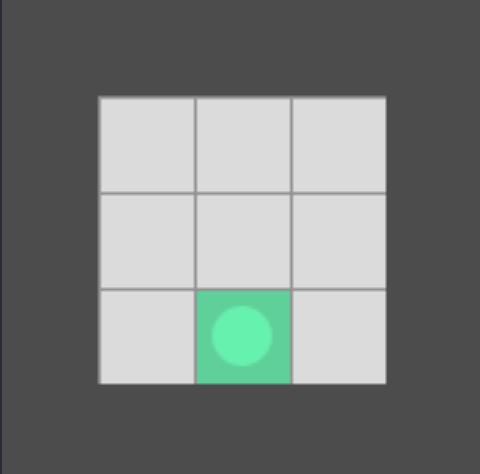
\includegraphics[width=1\linewidth]{1-agent-easy.png}\\
    \captionof{figure}[One Agent in a 5x5 Environment]{Visualization of a small environment with one agent}\label{fig:1-easy}
  \end{minipage}
  \hfill
  \begin{minipage}[b]{0.69\textwidth}
    \centering
    \begin{tabular}{lc}\hline
      Setting & Fully colored \\ \hline
        1 ppo & 3383 \\
        1 dqn & 650 \\ \hline
      \end{tabular}
      \captionof{table}[Training Results of one Agent in a 5x5 Environment]{Number of times the agent fully colored the environment during training with each learning algorithm \\}\label{t:1-easy}
    \end{minipage}
  \end{minipage}\\\\

Table \ref{t:1-easy} shows the amount of times the grid on the left (Figure \ref{fig:1-easy}) was fully colored by one agent using each learning algorithm during approximately 80.000 \verb|--frames|. The PPO agent colored the whole grid a total amount of 3383 times and the DQN agent 650 times. This means that at least 3383 PPO and 650 DQN episodes were played through. A fixed upper episode number does not exist, since it depends on the amount of steps agents need to reach the goal. The less they need, the more episodes they could play. The 80.000 frames are an approximation of the overall step count the agents can execute. The number of goals is a way to compare similar executions, and will be used as a general score to filter the best settings of the 70 executions.

\begin{figure}[hpbt]
    \centering
    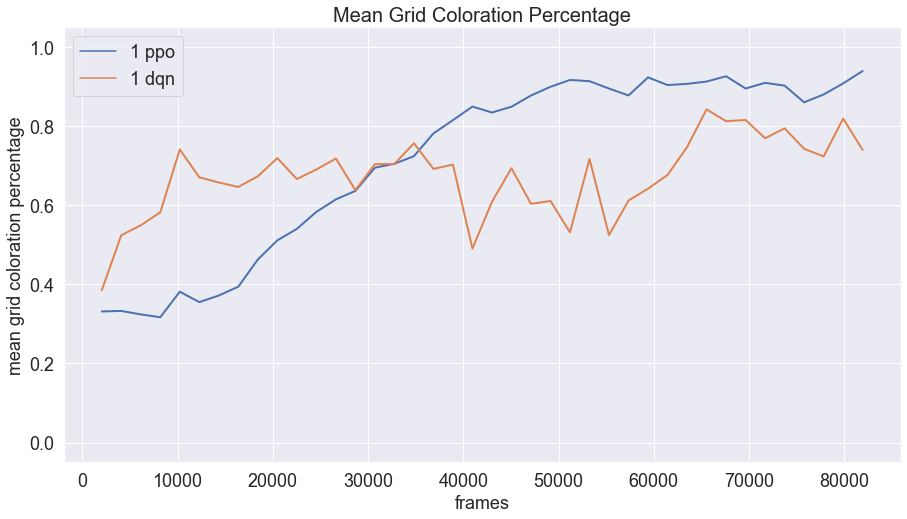
\includegraphics[width=0.8\textwidth]{1-easy-plot.png}\\
    \caption[Mean Coloration Percentage of one Agent in a 5x5 Environment]{The mean coloration percentage in a 5x5 grid and one acting agent}\label{fig:1-easy-plot}
\end{figure}

The average grid coloration percentage during the training is shown in plot \ref{fig:1-easy-plot}. The plot lines start at around 2048 frames, since this marks the first time an entry is saved. This specific number originates from the 128 \verb|--frames-per-proc| with \verb|proc| referencing the parallel environments. This in turns means that 128 steps in 16 environments are executed. During those 128 steps, with 10 \verb|--max-steps| in the worst case, 12 episodes could be completed in each environment. All data of such completed episodes are gathered and mean values are calculated. 

The plot depicts the average grid coloration percentage of the end of completed episodes. For the DQN line, this means, that the first entry at 2048 frames contains a final mean grid coloration of 40\%. The plot also exceeds the 80.000 default \verb|--frames|, since the last data entry includes the last 2048 frames. This and more training plots are shown in Appendix \ref{ax:plots}.

Plots and tables that refer to the fully colored grid values is the only case, in which the occurrences are counted instead of calculating mean values. 
Hence, in the table \ref{t:1-easy} the total sum of all finished episodes with a fully colored grid is presented.
Both training runs solve the environment and the plot illustrates that in both cases, a high percentage of the grid is colored. The DQN execution yields a better performance in the early stage, whereas the PPO agent gradually improves over time. In both cases, an average final coloration of over 70\% is eventually reached. This concludes that the grid is solvable with the default parameters.

\section{Easy Setup} \label{easy_env}

Now the multiagent scenario is compared. A set of two agents are trained to color the field of the same default dimensions, see Figure \ref{fig:2-coop-easy}. However, every agent executes an action during a step and with 10 steps and two agents in theory 20 cells could be visited. Hence, the \verb|--max-steps| count is reduced to eight. This should leave enough space for agents to make mistakes and still have a chance to solve the grid.

In order to get an overview of the overall 70 training results, the remaining 68 multiagent executions are divided into three different \verb|--setting| values. The first data division only covers the cooperation compositions, including ``difference-reward''. Table \ref{t:2-coop-easy} illustrates the scoreboard of the top three executions in this specification for each learning algorithm, measured by the total amount of complete colorations. \\\\

\begin{minipage}{\textwidth}
  \begin{minipage}[b]{0.29\textwidth}
    \centering
    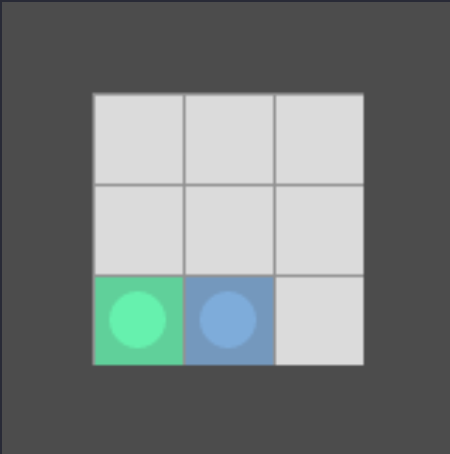
\includegraphics[width=1\linewidth]{2-agents-easy.png}\\
    \captionof{figure}[Two Agents in a 5x5 Environment]{Visualization of a small environment with two agents}\label{fig:2-coop-easy}
  \end{minipage}
  \hfill
    \begin{minipage}[b]{0.69\textwidth}
    \centering
    \begin{tabular}{clc}\hline
         & Top PPO Cooperation Settings & Fully colored \\ \hline
        {\small 1} & cooperation difference-reward & 1683 \\
        {\small 2} & cooperation & 1109 \\
        {\small 3} & cooperation sm-goal-no-reset & 533 \\ \hline
         &   \\ \hline
         & Top DQN Cooperation Settings & Fully colored \\ \hline
        {\small 1} & cooperation difference-reward & 5949 \\
        {\small 2} & cooperation am-goal-no-debt & 3197 \\
        {\small 3} & cooperation am-goal & 2880 \\ \hline
        \end{tabular}
        \captionof{table}[Top Training Results of two Cooperation Agents in a 5x5 Environment]{Number of times two agents working in cooperation fully colored the environment during training.\\}\label{t:2-coop-easy}
    \end{minipage}
  \end{minipage}\\\\

In both cases, the agents with the DR setting scored best, 1683 times with the PPO algorithm and 5949 times by using DQN. The PPO scores continue with the default cooperation scenario on second and the SM with the ``goal-no-reset'' condition on third place. On the contrary, the DQN results show AM settings on the remaining places, with the additions ``goal-no-debt'' on second place and ``goal'' on the third place. It is visible that in both scoreboards the second and third executions are far behind the corresponding DR setting in terms of fully coloration counts.

\begin{figure}[hpbt]
    \centering
    \subfloat[Reward summary of PPO agents]{
        \label{fig:2-ppo-coop-easy} 
        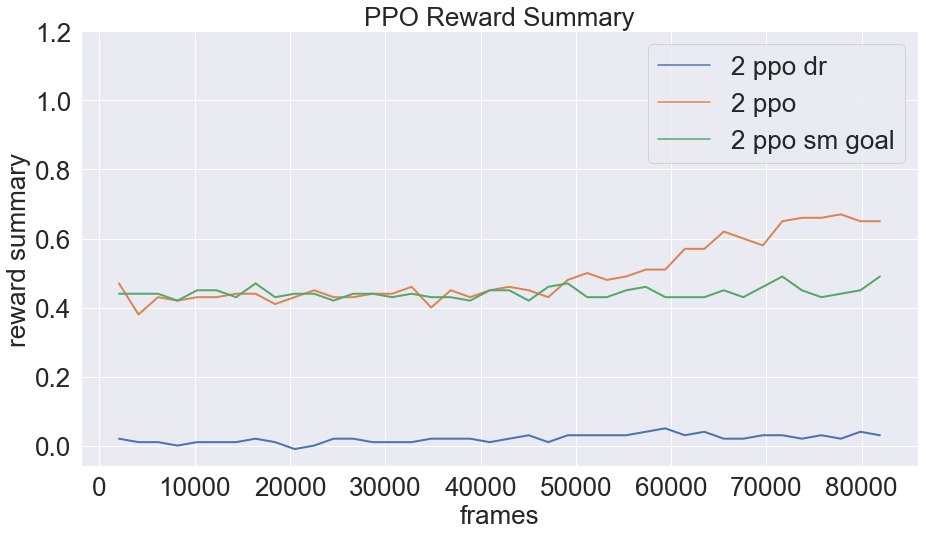
\includegraphics[width=0.48\linewidth]{2-ppo-easy.png}}
    \hspace{0.01\textwidth}
    \subfloat[Reward summary of DQN agents]{
        \label{fig:2-dqn-coop-easy} 
        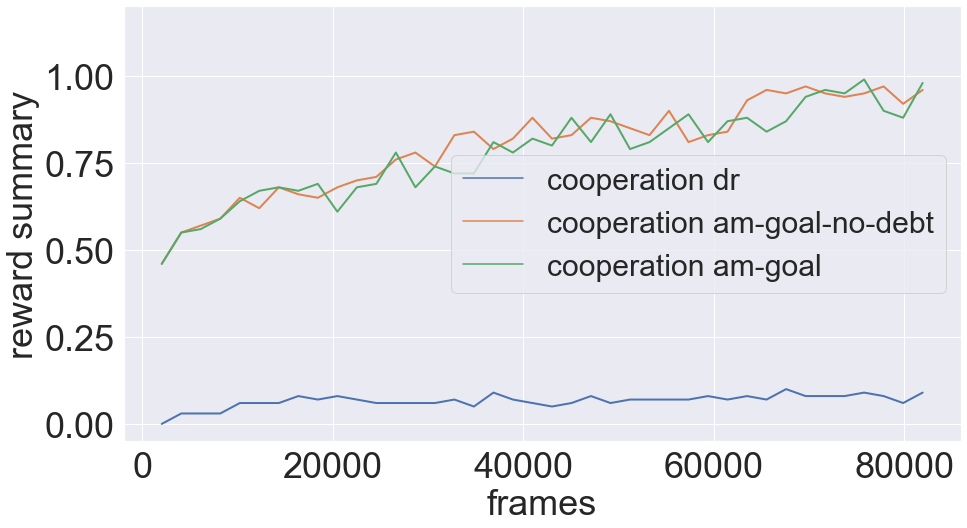
\includegraphics[width=0.48\linewidth]{2-dqn-easy.png}}
    \caption[Reward Summaries of the Top Cooperation Modes in a 5x5 Environment]{Reward Summaries of the top three cooperation compositions using PPO (left) and DQN (right)}
    \label{fig:multipic_plots_coop_easy} 
\end{figure}

In the two plots of Figure \ref{fig:multipic_plots_coop_easy}, the reward summary of the top scores are displayed (see table \ref{t:2-coop-easy}). The term reward summary is used, since the rewards of cooperating agents are equal and sometimes contain only slight changes through markets. However, in other agent compositions, the rewards are rather specific to each agents' contribution. In any case, the logged training data contains the mean reward of every agent separately. 

In order to summarize cooperation rewards, the average value of those separate agent rewards is calculated for each data entry and the results are then plotted here. For reward summaries of all other compositions, each data entry is summarized with the sum of the separate agent rewards. The maximum y-axis label is set to 1.2, since agents get a reward of one, if they color the whole field, and additionally could get a reward of 0.1 for the final step. Through the reward summary calculations rounding errors may occur, which could in turn exceed the maximum reward of 1.1. Furthermore, markets could also contribute to bigger rewards. 

Even though, the executions with the DR configuration scored highest in terms of reaching the goal, the reward lines in this case stay around 0.1. The reason for that is that agents get the difference of two rewards, leading to very small values. All rewards, except the DRs, show a continuous increase and at least reach a summary reward of 0.8. 

The next training executions to look at are ``mixed-motive'' settings. Again, a scoreboard listing the top three results of each learning algorithm, is shown in table \ref{t:2-mixed-easy}.
\begin{center}
    \begin{tabular}{clc}\hline
         & Top PPO Mixed-Motive Settings & Fully colored \\ \hline
        {\small 1} & mixed-motive & 1734 \\
        {\small 2} & mixed-motive sm-no-reset & 1422 \\
        {\small 3} & mixed-motive sm-goal-no-reset & 1377 \\ \hline
         &   \\ \hline
         & Top DQN Mixed-Motive Settings & Fully colored \\ \hline
        {\small 1} & mixed-motive sm & 5417 \\
        {\small 2} & mixed-motive am-no-reset & 5379 \\
        {\small 3} & mixed-motive sm-goal & 5302 \\ \hline
        \end{tabular}
        \captionof{table}[Top Training Results of two Mixed-Motive Agents in a 5x5 Environment]{Number of times two agents working in a mixed-motive setting fully colored the environment during training.}\label{t:2-mixed-easy}
    \end{center}

The PPO scoreboard shows that the plain ``mixed-motive'' setting is on the top with a score of 1734. Subsequently, SM configurations follow, with the addition of ``no-reset'' on second and ``goal-no-reset'' on third place. The DQN scores also show two SM settings, the default market occupies the first place and the SM with the ``goal'' addition is on the last place, both however colored the grid a total of over 5300 times. The AM with the ``no-reset'' condition is on the second place in the DQN statistics.

\begin{figure}[hpbt]
    \centering
    \subfloat[Mean trades of PPO agents]{
        \label{fig:2-ppo-mixed-easy} 
        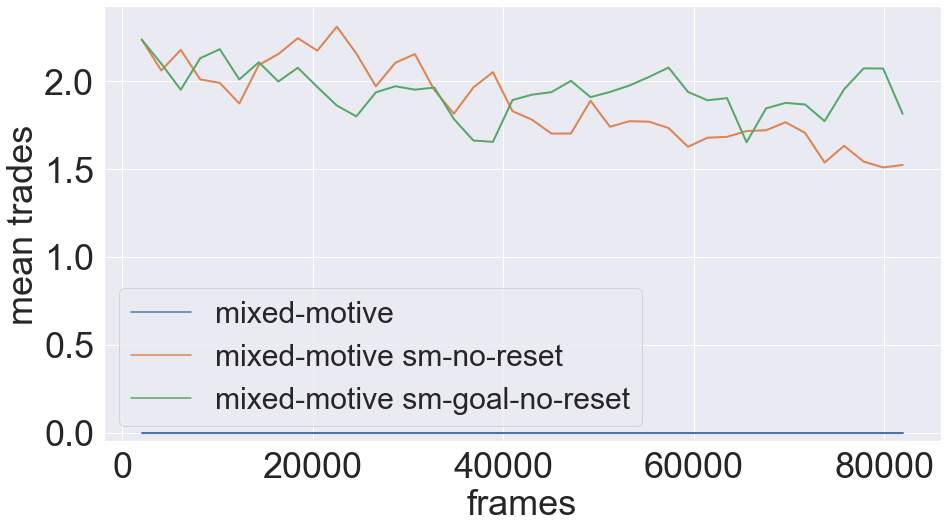
\includegraphics[width=0.48\linewidth]{2-ppo-mixed-easy.png}}
    \hspace{0.01\textwidth}
    \subfloat[Mean trades of DQN agents]{
        \label{fig:2-dqn-mixed-easy} 
        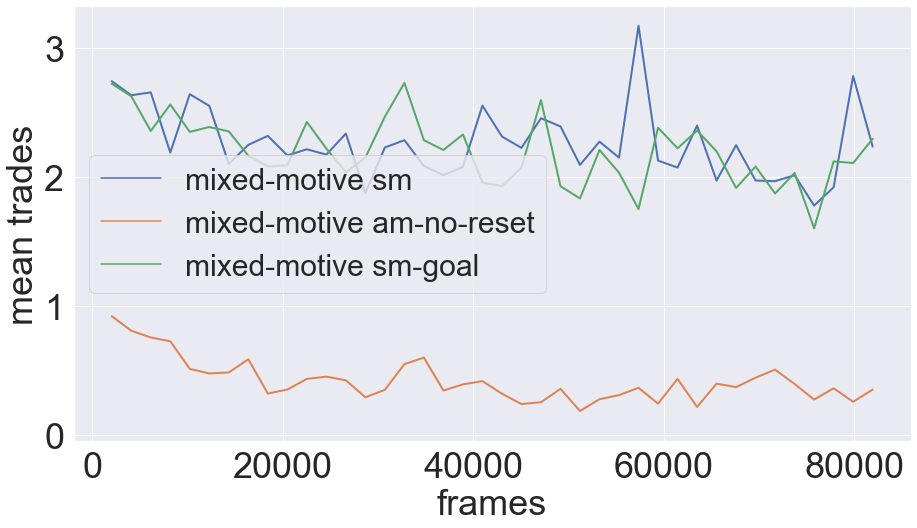
\includegraphics[width=0.48\linewidth]{2-dqn-mixed-easy.png}}
    \caption[Mean Trades of the Top Mixed-Motive Modes in a 5x5 Environment]{Mean trades of the top three mixed-motive compositions using PPO (left) and DQN (right)}
    \label{fig:multipic_plots_mixed_easy}
\end{figure}

In Figure \ref{fig:multipic_plots_mixed_easy}, two plots are shown, visualizing the trading behavior of the agents during training. The plots display the mean amount of trades in the parallel environments. In plot \ref{fig:2-ppo-mixed-easy}, the blue line stays at zero, since this execution does not contain a market extension. The other two lines are slightly decreasing and move between 2.2 and 1.5. Both lines represent a SM interaction with the values showing that on average two market transactions occurred. This in turn means that about two shares were bought in the completed episodes of all parallel environments.

In the right plot \ref{fig:2-dqn-mixed-easy}, an AM is represented with the orange line. The mean trades are less compared to the other two SM lines. This is often the case for the two markets, since action purchases subtract a bigger value at once, whereas selling shares reduces a minor value of the payout continuously. Comparing the SM executions between PPO and DQN shows, that the restriction of ``no-reset'' lowers the average trades to around two, whereas without this specific condition the trade count is between two and three.

The last dataset division only includes executions of competitive agent compositions. Table \ref{t:2-comp-easy} shows the scoreboards of this setup.

\begin{center}
    \begin{tabular}{clc}\hline
         & Top PPO Competitive Settings & Fully colored \\ \hline
        {\small 1} & competitive sm-goal-no-reset & 3614 \\
        {\small 2} & competitive & 3461 \\
        {\small 3} & competitive sm-goal & 3225 \\ \hline
         &   \\ \hline
         & Top DQN Competitive Settings & Fully colored \\ \hline
        {\small 1} & competitive sm-goal-no-reset & 7877 \\
        {\small 2} & competitive sm & 7842 \\
        {\small 3} & competitive am-goal-no-debt & 7560 \\ \hline
        \end{tabular}
        \captionof{table}[Top Training Results of two Competitive Agents in a 5x5 Environment]{Number of times two agents working in a competitive setting fully colored the environment during training.}\label{t:2-comp-easy}
    \end{center}

For both learning algorithms, the most fully colored grids result from executions specifying a SM with the condition ``goal-no-reset''. In the DQN table the execution using the standard SM follows on second place and the last place is occupied by an AM with the specification ``goal-no-debt''. For PPO, however, the second place is the normal competitive mode without any additions and on third place is a SM execution with the ``goal'' restriction. Overall, the score differences within the tables are not significant, at most a difference of around 300 goal states is observed. Furthermore, the scores of the first places in these two boards are the best values achieved by a multiagent setup so far, with 3614 fully colored grids in the PPO table and 7877 in the DQN table.

\begin{figure}[hpbt]
    \centering
    \subfloat[Mean number of reset fields of PPO agents]{
        \label{fig:2-ppo-comp-easy} 
        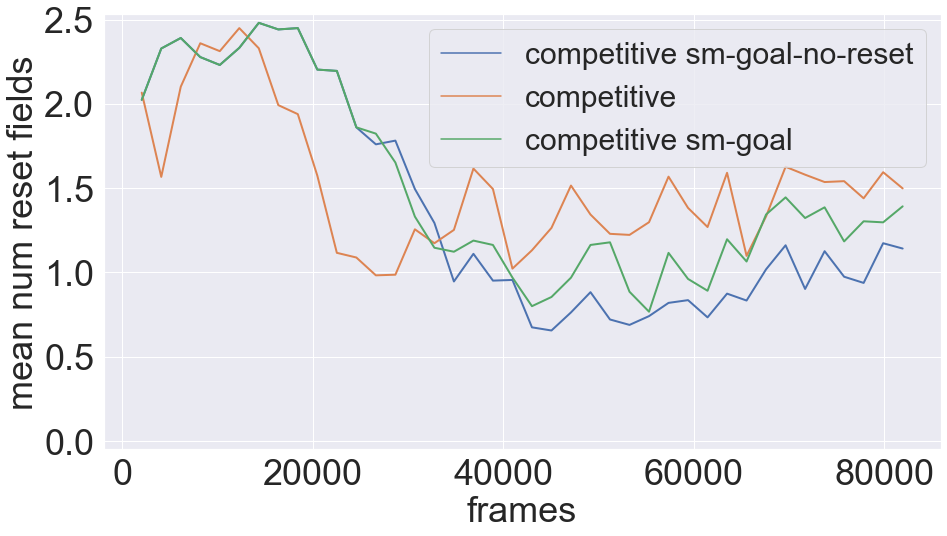
\includegraphics[width=0.48\linewidth]{2-ppo-comp-easy.png}}
    \hspace{0.01\textwidth}
    \subfloat[Mean number of reset fields of DQN agents]{
        \label{fig:2-dqn-comp-easy} 
        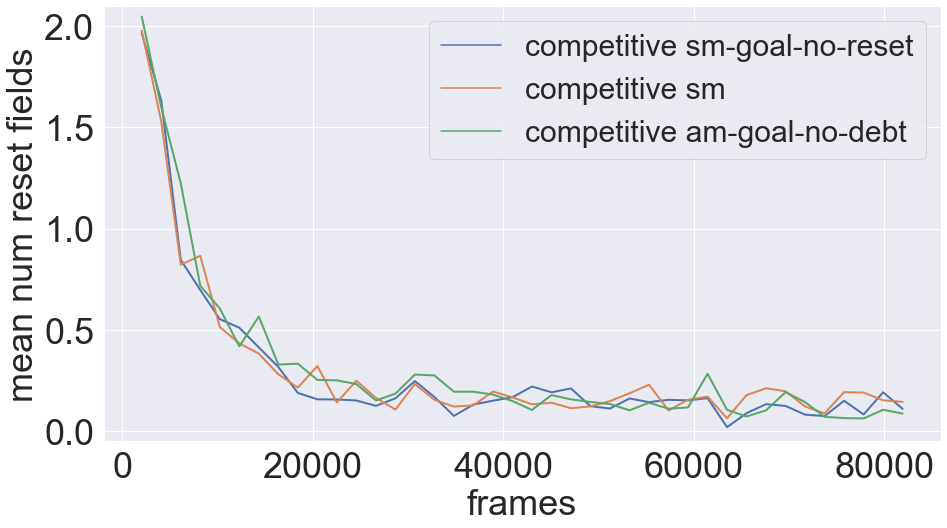
\includegraphics[width=0.48\linewidth]{2-dqn-comp-easy.png}}
    \caption[Mean Number of Reset Fields of the Top Competitive Modes in a 5x5 Environment]{Mean number of reset fields of the top three competitive compositions using PPO (left) and DQN (right)}
    \label{fig:multipic_plots_comp_easy}
\end{figure}

The plots to those scoreboards are displayed in Figure \ref{fig:multipic_plots_comp_easy}. In this case, the average amount of reset fields are visualized. All lines start at a value two, which means, that during the first 2048 frames an average of two cells are reset during the completed episodes. In both cases the graphs eventually drop, however for PPO executions this takes around 20.000 frames and in the later half a small increase in all lines can be observed. Meanwhile, the three DQN trainings rapidly reduce the average resets to around 0.3. This value is never reached by PPO executions, here the lowest score is approximately 0.6.

\section{Difficult Setup} \label{difficult_env}
To see how the results change when it becomes more challenging to reach the goal, all top executions shown before are now repeated in a bigger environment. The grid size is increased to seven, which provides an area of 25 cells for the agents to color. Also, since the grid offers more room, the amount of agents is increased to three.

To give the agents more time to learn, the \verb|--frames| are set to 200.000 and the value of \verb|--frames-per-proc| is changed to 256. With the increase to 256, the training data entries are now 4096 frames apart instead of the 2048 before. The number 4096 comes from multiplying the number of environments with the \verb|--frames-per-proc|. To successfully solve the grid with one agent, some DQN specific parameters needed to be tuned. As a result, the adjusted values of \verb|--replay-size|, \verb|--epsilon-decay| and \verb|--target-update| are 700.000, 20.000 and 10.000. 

In Figure \ref{fig:1-hard}, the one agent learning scenario during training in a difficult setup is shown. The agent view size is also noticeable, with the lighter floor and wall colors three tiles around the agent. In this case, the agent cannot see the two top rows of the grid. This, of course, also contributes to the difficulty of this setup. \\

\begin{minipage}{\textwidth}
  \begin{minipage}[b]{0.29\textwidth}
    \centering
    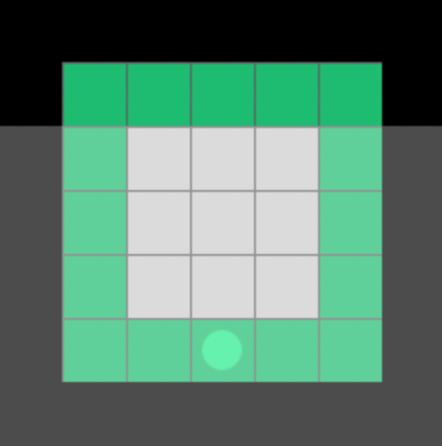
\includegraphics[width=1\linewidth]{1-agent-hard.png}\\
    \captionof{figure}[One Agent in a 7x7 Environment]{Visualization of a 7x7 Environment with one agent}\label{fig:1-hard}
  \end{minipage}
  \hfill
  \begin{minipage}[b]{0.69\textwidth}
    \centering
    \begin{tabular}{lc}\hline
      Setting & Fully colored \\ \hline
        1 ppo & 2924 \\
        1 dqn & 394 \\ \hline
      \end{tabular}
      \captionof{table}[Training Results of one Agent in a 7x7 Environment]{Number of times the agent fully colored the environment during training with each learning algorithm.\\ }\label{t:1-hard}
    \end{minipage}
  \end{minipage}\\\\

The results of the training executions with one agent are shown in table \ref{t:1-hard}. In this case, the maximum step amount is again the default value of 49, since the grid size of seven is squared. Similar to the easier setup, the PPO training yields more fully colored grids compared to the DQN execution. While the PPO agent reaches the goal 2924 times, the DQN agent only achieves 394 goal states. Comparing those numbers with their corresponding easy equivalent, it is also obvious that the scores of both learning algorithms have decreased.

\begin{figure}[hpbt]
    \centering
    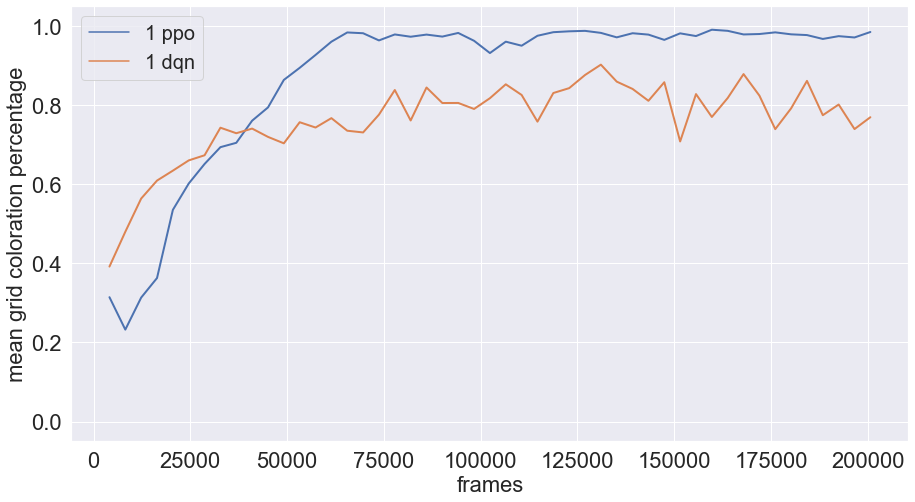
\includegraphics[width=0.8\textwidth]{1-hard-plot.png}\\
    \caption[Mean Coloration Percentage of one Agent in a 7x7 Environment]{The mean coloration percentage of a 7x7 grid and one acting agent}\label{fig:1-hard-plot}
\end{figure}

Looking at the mean coloration percentage plot \ref{fig:1-hard-plot} however, both executions show an increase to a relatively high percentage. The DQN agent training reaches an average of 80\% grid coloration with only minor deviations. In comparison, the training with PPO has a steep incline from 20\% to 95\% and after 60.000 frames, this high percentage is maintained until the end of training. This proves that both algorithms learned strategies to color the environment with the set parameters.

For the training in this setting with three agents, the maximum step amount is set to 20. In Figure \ref{fig:3-hard}, a training frame is visualized. In this time step, the observation of the top agent does not include the two agents on the bottom. The two agents in turn also cannot see the top agent, but are aware of their neighbor. 

The results of the cooperation executions with three agents are listed in table \ref{t:3-coop-hard}. \\

\begin{minipage}{\textwidth}
  \begin{minipage}[b]{0.29\textwidth}
    \centering
    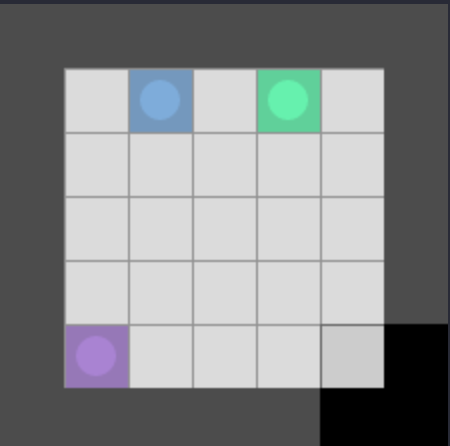
\includegraphics[width=1\linewidth]{3-agents-hard.png}\\
    \captionof{figure}[Three Agents in a 7x7 Environment]{Visualization of a 7x7 environment with three agents}\label{fig:3-hard}
  \end{minipage}
  \hfill
    \begin{minipage}[b]{0.69\textwidth}
    \centering
    \begin{tabular}{clc}\hline
         & Top PPO Cooperation Settings & Fully colored \\ \hline
        {\small1} & cooperation difference-reward & 166 \\
        {\small2} & cooperation & 10 \\
        {\small3} & cooperation sm-goal-no-reset & 0 \\ \hline
         &   \\ \hline
         & Top DQN Cooperation Settings & Fully colored \\ \hline
        {\small 1} & cooperation difference-reward & 115 \\
        {\small 2} & cooperation am-goal-no-debt & 0 \\
        {\small 3} & cooperation am-goal & 0 \\ \hline
        \end{tabular}
        \captionof{table}[Top Training Results of three Cooperation Agents in a 7x7 Environment]{Number of times three agents working in cooperation fully colored the environment during training. \\}\label{t:3-coop-hard}
    \end{minipage}
  \end{minipage}

\begin{figure}[hpbt]
    \centering
    \subfloat[Mean coloration percentage of PPO agents]{
        \label{fig:3-ppo-coop-hard} 
        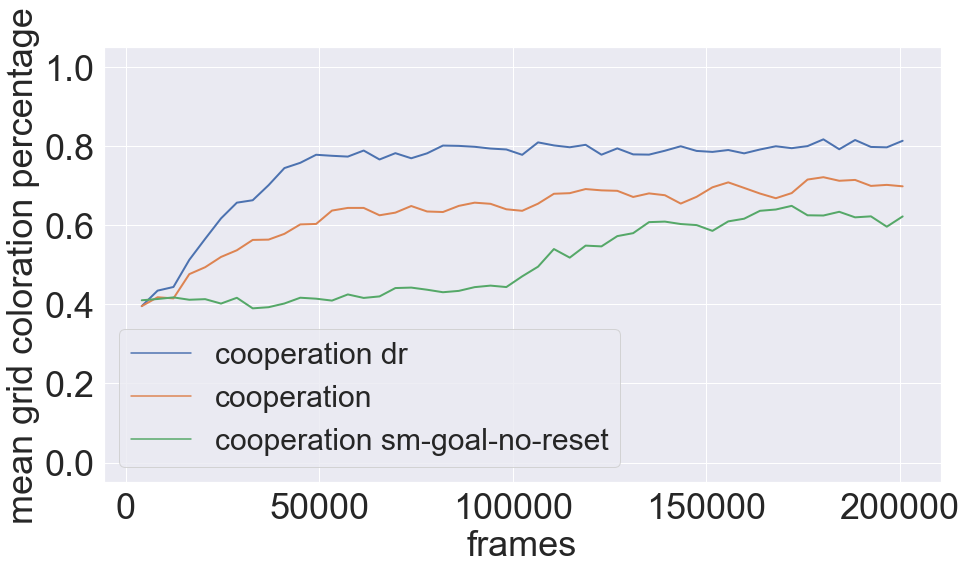
\includegraphics[width=0.48\linewidth]{3-ppo-coop-hard.png}}
    \hspace{0.01\textwidth}
    \subfloat[Mean coloration percentage of DQN agents]{
        \label{fig:3-dqn-coop-hard} 
        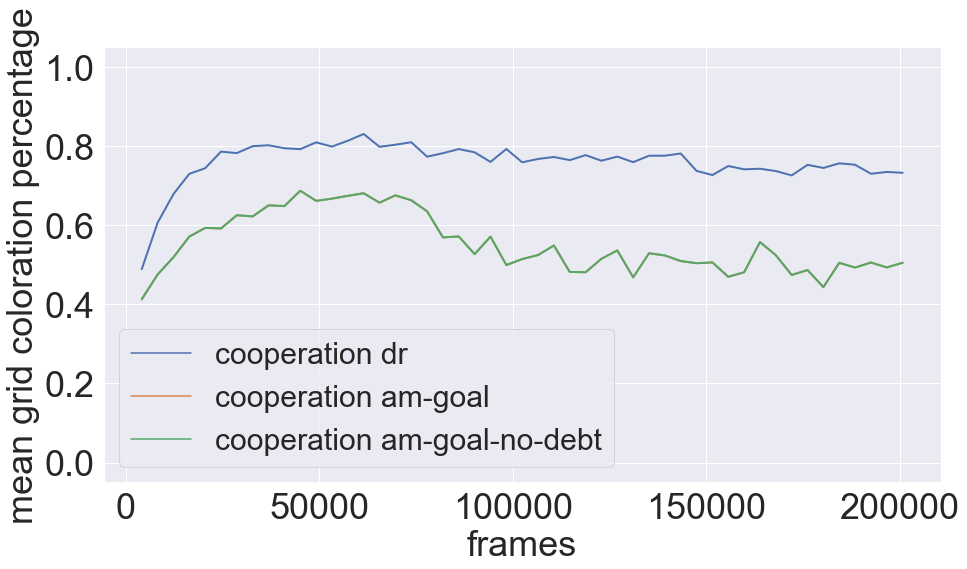
\includegraphics[width=0.48\linewidth]{3-dqn-coop-hard.png}}
    \caption[Mean Coloration Percentage of the Top Cooperation Modes in a 7x7 Environment]{Mean grid coloration percentages of the top three cooperation compositions using PPO (left) and DQN (right)}
    \label{fig:multipic_plots_coop_hard}
\end{figure}

This table shows that all cooperative settings with specified markets yielded no goal achievements. In the DQN scoreboard, only the DR approach resulted in 115 complete colorations. The PPO table also lists the DR training result as first place with a total score of 166. The standard cooperation training ranks second in this regard, but only with 10 fully colored states. Overall, the scores have significantly decreased in comparison to the small environment results.

In the plots of Figure \ref{fig:multipic_plots_coop_hard}, it is visible that both DR trainings result in a similar average coloration percentage of around 80\%. In the DQN plot, only two lines are visible due to the ``goal'' addition of the market execution. Since the goal is never reached, the final market payout with the trading matrix could not be applied. Hence, both trainings yielded the same decisions and overlap in this graph. 

\begin{center}
\begin{tabular}{clc}\hline
      & Top PPO Mixed-Motive Settings & Fully colored \\ \hline
    {\small 1} & mixed-motive & 247 \\
    {\small 2} & mixed-motive sm-goal-no-reset & 133 \\
    {\small 3} & mixed-motive sm-no-reset & 66 \\ \hline
      &   \\ \hline
      & Top DQN Mixed-Motive Settings & Fully colored \\ \hline
    {\small 1} & mixed-motive sm-goal & 116 \\
    {\small 2} & mixed-motive sm & 42 \\
    {\small 3} & mixed-motive am-no-reset & 31 \\ \hline
    \end{tabular}
    \captionof{table}[Top Training Results of three Mixed-Motive Agents in a 7x7 Environment]{Number of times three agents working in a mixed-motive setting fully colored the environment during training.}\label{t:3-mixed-hard}
\end{center}

\begin{figure}[hpbt]
    \centering
    \subfloat[Fully colored grid achievements of PPO agents]{
        \label{fig:3-ppo-mixed-hard} 
        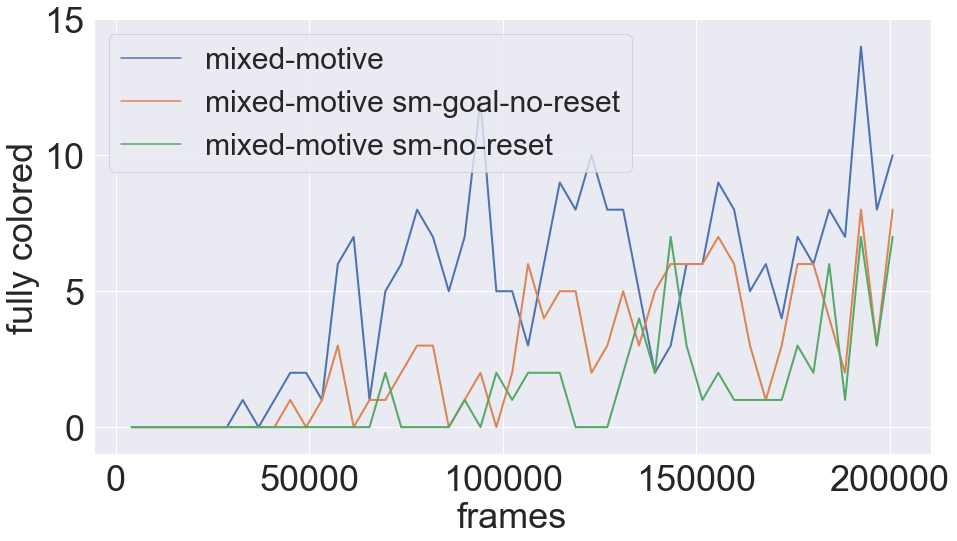
\includegraphics[width=0.48\linewidth]{3-ppo-mixed-hard.png}}
    \hspace{0.01\textwidth}
    \subfloat[Fully colored grid achievements of DQN agents]{
        \label{fig:3-dqn-mixed-hard} 
        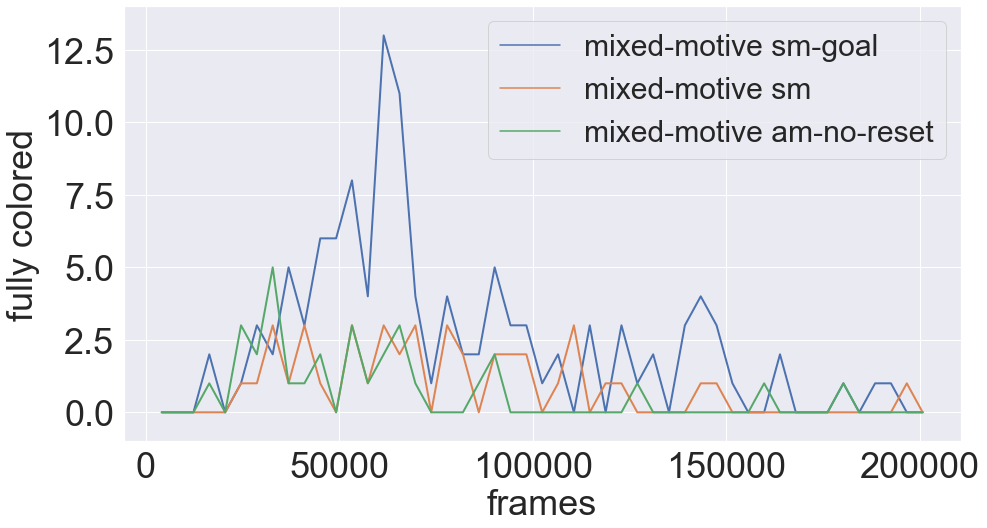
\includegraphics[width=0.48\linewidth]{3-dqn-mixed-hard.png}}
    \caption[Plots of fully coloration achievements of the Top Mixed-Motive Modes in a 7x7 Environment]{Environment goal achievements of the top three mixed-motive compositions using PPO (left) and DQN (right)}
    \label{fig:multipic_plots_mixed_hard}
\end{figure}

Continuing with the mixed-motive executions, table \ref{t:3-mixed-hard} shows the goal achievements.
The PPO board still has the default mixed-motive composition on first place, with 247 fully colored counts. Comparing this board with the results of the smaller environment, it is clear that the next two position have swapped places. Also in the DQN board, the order has changed. The previous last placed ``sm-goal'' setting is now on the first place with 116 colorations and the other two executions moved down. 

Figure \ref{fig:multipic_plots_mixed_hard} displays the two plots that show how the fully coloration numbers are generated. On the left-hand side, the PPO based trainings show an increase of reaching the goal state towards the end, with a maximum of around 14. This means, that in a data point, which extracts over 4096 frames and 16 parallel environments 14 episodes ended with the grid fully colored. Looking at the DQN plots it is evident that the highest point of the learning curve lies at approximately 60.000 frames and then it levels off.

\begin{center}
\begin{tabular}{clc}\hline
      & Top PPO Competitive Settings & Fully colored \\ \hline
    {\small 1} & competitive & 277 \\
    {\small 2} & competitive sm-goal & 165 \\
    {\small 3} & competitive sm-goal-no-reset & 111 \\ \hline
      &   \\ \hline
      & Top DQN Competitive Settings & Fully colored \\ \hline
    {\small 1} & competitive sm-goal-no-reset & 367 \\
    {\small 2} & competitive sm & 240 \\
    {\small 3} & competitive am-goal-no-debt & 198 \\ \hline
    \end{tabular}
    \captionof{table}[Top Training Results of three Competitive Agents in a 7x7 Environment]{Number of times three agents working in a competitive setting fully colored the environment during training.}\label{t:3-comp-hard}
\end{center}

Finally, the last table \ref{t:3-comp-hard} shows the top scores of competitive compositions in a seven by seven coloration environment. While up to this point the first places of PPO executions in the difficult setting resulted in higher scores than their DQN counterparts, in this table this is not the case. The top competitive DQN training resulted in 367 completely colored fields, whereas the highest PPO score is only 277. Furthermore, the order of the DQN board stayed the same, while the PPO scores changed, with the previous first placed ``sm-goal-no-reset'' now being on the last place. 

\begin{figure}[hpbt]
    \centering
    \subfloat[Mean trades of PPO agents]{
        \label{fig:3-ppo-comp-hard} 
        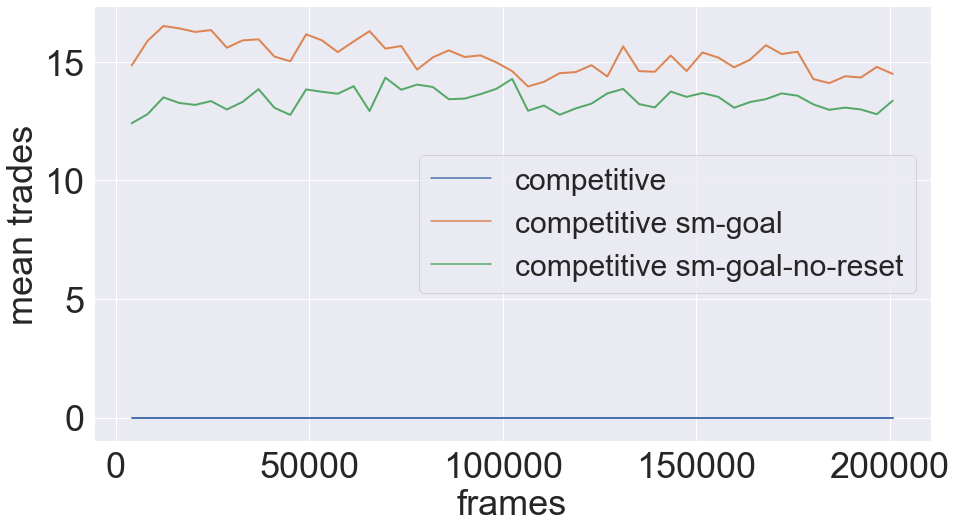
\includegraphics[width=0.48\linewidth]{3-ppo-comp-hard.png}}
    \hspace{0.01\textwidth}
    \subfloat[Mean trades of DQN agents]{
        \label{fig:3-dqn-comp-hard} 
        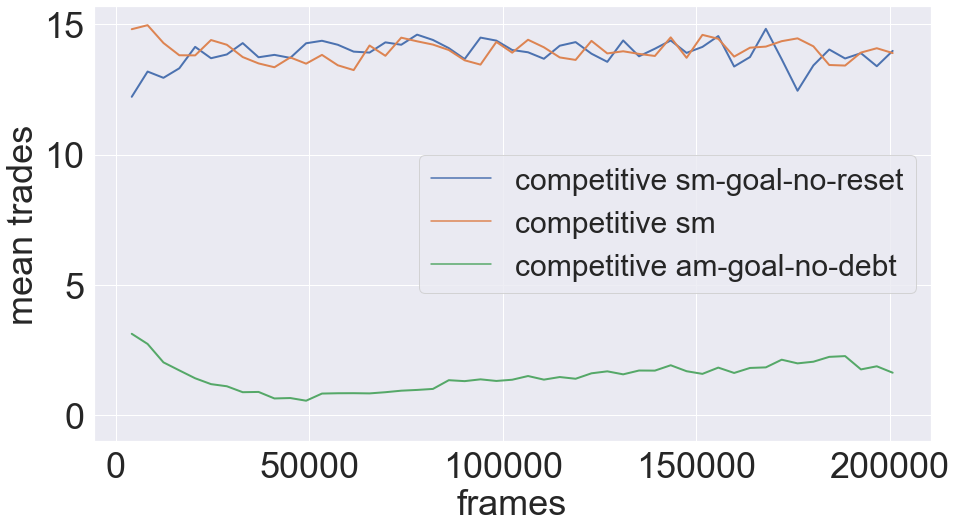
\includegraphics[width=0.48\linewidth]{3-dqn-comp-hard.png}}
    \caption[Mean Trades of the Top Competitive Modes in a 7x7 Environment]{Mean trades of the top three competitive compositions using PPO (left) and DQN (right)}
    \label{fig:multipic_plots_comp_hard} 
\end{figure}

The last thing to point out are the mean trade counts in those trainings. Plot \ref{fig:3-ppo-comp-hard} and \ref{fig:3-dqn-comp-hard} display how many market transactions on average were executed. The two plots show similarities of building the strategy to sell around 15 shares on average. For the AM in the DQN execution the mean amount is only at approximately 3 trades. \\\\

\section{Rooms Setup}\label{room_env}
To further stress test the learning abilities of agents, the environment is now also divided into rooms. In order to set up a reasonable room division, the environment size needed to be increased to a 9x9 grid. A visualization of this setting is shown in Figure \ref{fig:1-agent-rooms}. The maximum step count in trainings with one agent is, again, not set manually, which results in 81. Other than changing the \verb|--env| parameter to ``FourRooms-Grid-v0'' and the grid size to 9 the same parameters of the previous seven by seven settings were used. \\

\begin{minipage}{\textwidth}
  \begin{minipage}[b]{0.29\textwidth}
    \centering
    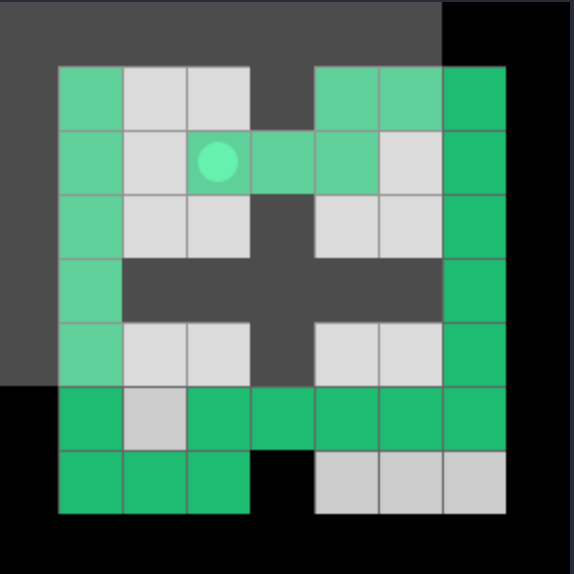
\includegraphics[width=1\linewidth]{1-agent-rooms.png}\\
    \captionof{figure}[One Agent in a 9x9 Rooms Environment]{Visualiza- tion of an environment with rooms and one agent}\label{fig:1-agent-rooms}
  \end{minipage}
  \hfill
  \begin{minipage}[b]{0.69\textwidth}
    \centering
    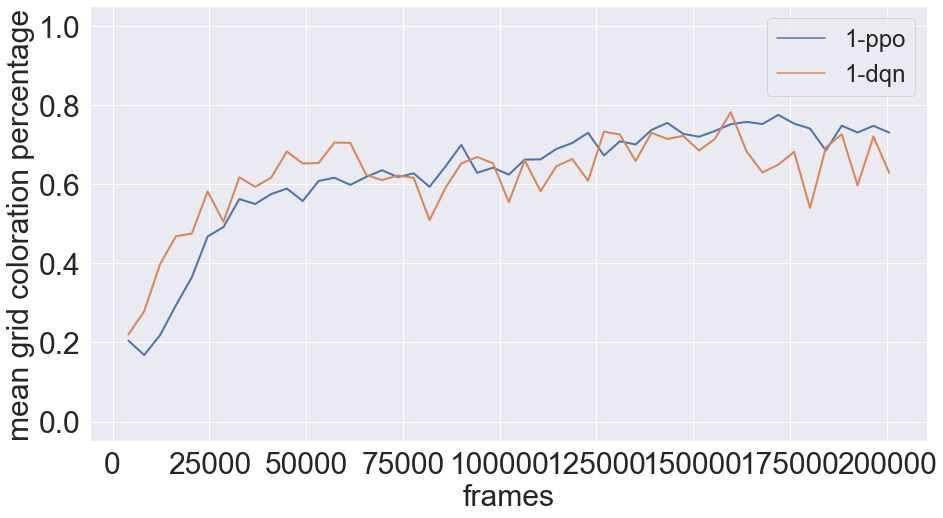
\includegraphics[width=1\linewidth]{1-rooms-plot.png}\\
    \captionof{figure}[Mean Coloration Percentage of one Agent in a 9x9 Rooms Environment]{The mean coloration percentage in a 9x9 Rooms Environment and one acting agent \\}\label{fig:1-rooms-plot}
    \end{minipage}
  \end{minipage}\\\\

Figure \ref{fig:1-rooms-plot} replaces the score table, since both ppo and dqn trainings with one agent never reached the goal. However, the plot shows potential, due to the increase from 20\% average coloration to around 70\%.

\begin{figure}[hpbt]
    \centering
    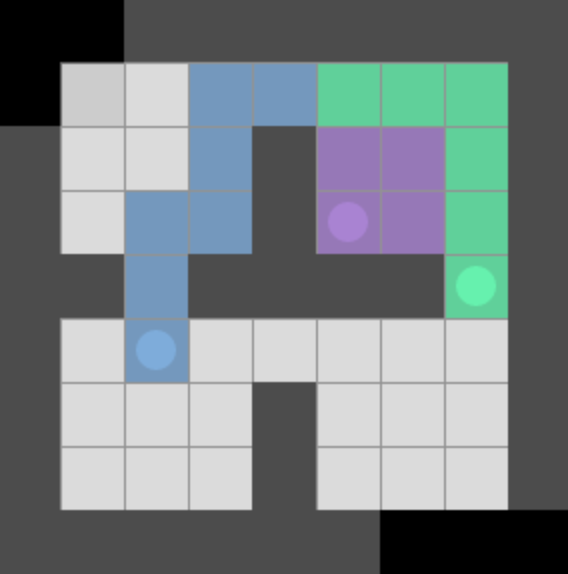
\includegraphics[width=0.3\textwidth]{3-agents-rooms.png}\\
    \caption[Three Agents in a 9x9 Rooms Environment]{Visualization of an environment with rooms and three agents}\label{fig:3-agents-rooms}
\end{figure}

For the multiagent training with three agents, the step amount is set to 30. A visualization of this setup is shown in Figure \ref{fig:3-agents-rooms}. Furthermore, only the first places of the scoreboards of chapter \ref{difficult_env} were trained in this environment, because of long execution times. As a result these six settings are analyzed, for PPO:
\begin{itemize}
    \item cooperation dr
    \item mixed-motive
    \item competitive
\end{itemize}
    and for DQN:
\begin{itemize}
    \item cooperation dr
    \item mixed-motive sm-goal
    \item competitive sm-goal-no-reset.
\end{itemize}

Unfortunately, all but one of the training executions never fully colored the environment. Only the top DQN competitive training managed to reach the goal state a total of 10 times. In Figure \ref{fig:3-ppo-rooms}, it is shown that the PPO agents learn to color 70\% of the grid over time. In the DQN plot however, they reach the peak of 80\% early on and drop the coloration percentage slowly afterwards, with the lowest point in the DR setting to 40\%.  

\begin{figure}[hpbt]
    \centering
    \subfloat[Mean coloration percentage of PPO agents]{
        \label{fig:3-ppo-rooms}
        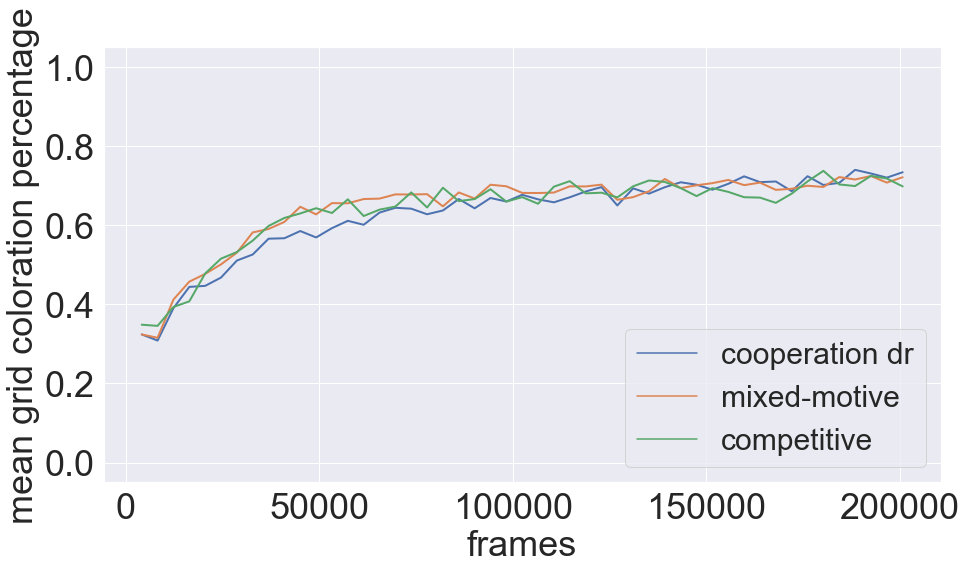
\includegraphics[width=0.48\linewidth]{3-ppo-rooms.png}}
    \hspace{0.01\textwidth}
    \subfloat[Mean coloration percentage of DQN agents]{
        \label{fig:3-dqn-rooms} 
        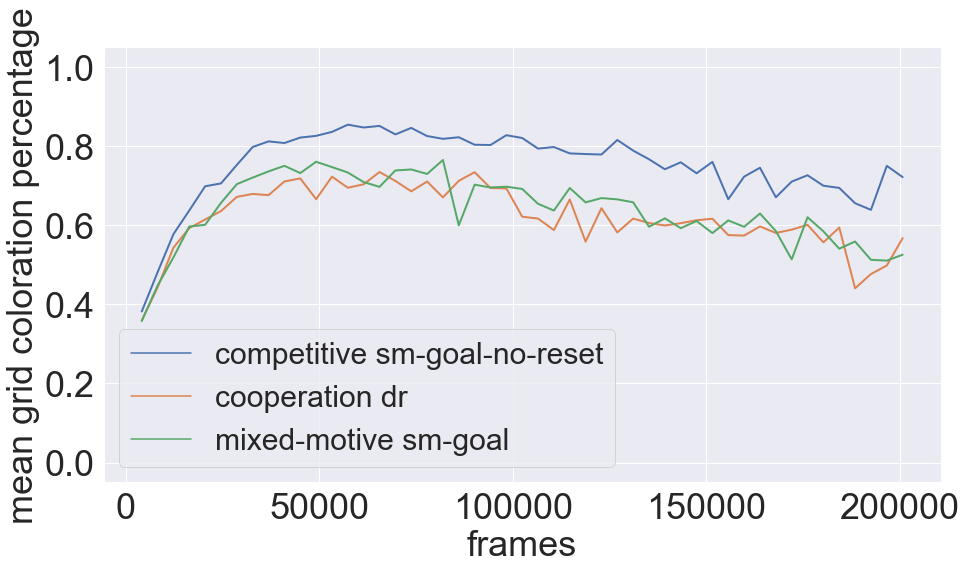
\includegraphics[width=0.48\linewidth]{3-dqn-rooms.png}}
    \caption[Mean Coloration Percentage of the Top Modes in a 9x9 Rooms Environment]{Mean grid coloration percentages in a 9x9 Rooms Environment using PPO (left) and DQN (right)}
    \label{fig:multipic_plots_rooms} 
\end{figure}